\documentclass[a4paper, 10pt]{scrartcl}

\usepackage[english]{babel}
\usepackage[stixtwo]{fontsetup}

\def\hmargin{15mm}
\def\vmargin{15mm}

\usepackage[
  left=\hmargin,
  right=\hmargin,
  top=\vmargin,
  bottom=\vmargin,
  % showframe,
]{geometry}

\usepackage{tikz}
\usetikzlibrary{calc}

\usepackage{enumitem}

\setlist[itemize]{noitemsep, topsep=3pt, partopsep=3pt, left=.67em}

\usepackage{xcolor}

\colorlet{light-red}{red!80}
\colorlet{dark-red}{red!40!black}
\colorlet{light-gray}{gray!20}
\colorlet{dark-gray}{black!60}

\usepackage{fontawesome}
\usepackage{array}
\usepackage{graphicx}
\usepackage{tabto}
\usepackage[
luatex,
colorlinks=true,
allcolors=black,
]{hyperref}
\usepackage{qrcode}

\def\leftcolumnwidth{.275\textwidth}
\def\rightcolumnwidth{.675\textwidth}

\setlength\parindent{0pt}
\setlength\parskip{.33em}
\setlength\fboxsep{0pt}

\newcommand{\resumesection}[1]{%
  \bgroup%
  \Large\bfseries\color{dark-gray}#1\par\vspace{-4mm}%
  \tikz{\draw[light-red, line width=0.75mm] (0,0) -- (\textwidth,0);}%
  \par\vspace{2mm}%
  \egroup%
}

\newcommand{\timedentry}[3]{%
  \bgroup%
  \bfseries#1 \hfill%
  \makebox[12mm][c]{#2} -- \makebox[12mm][c]{#3}%
  \egroup%
}

\begin{document}
\thispagestyle{empty}%
\sffamily%
%%% ------------------------------------------------------------------------ %%%
%%% ----------------------------- Overlay ----- ---------------------------- %%%
%%% ------------------------------------------------------------------------ %%%
\begin{tikzpicture}[overlay, remember picture]
	% Line between left and right column
	\draw[draw=light-gray, line width=1.5mm]
	($(current page.north west)+(\hmargin+.3\textwidth,-\vmargin)$) --
	($(current page.south west)+(\hmargin+.3\textwidth,\vmargin)$)
	;

	% Box for name + title
	\fill[fill=dark-gray]
	($(current page.north east)+(-\hmargin,-\vmargin)$) rectangle
	++(-\rightcolumnwidth,-2.5*\vmargin)
	node[midway, text width=\rightcolumnwidth, text=white, align=center]{
			\LARGE{}Tibor SÁNDOR\\
			\tikz{\draw[white, ultra thick] (0,0) -- (2,0);}\\[6mm]
			\large{}MSc Student in Mechatronics Engineering
		}
	;

	% Link at bottom left
	\node[anchor=south west, text=dark-gray, font=\footnotesize] at
	($(current page.south west)+(\hmargin,0)$)
	{${}^1$\url{https://www.conftool.net/sefi2024/index.php?page=browseSessions\&print=export\&ismobile=false\&form_session=604\#paperID432}}
	;
\end{tikzpicture}%
%%% ------------------------------------------------------------------------ %%%
%%% ----------------------------- Left Column ------------------------------ %%%
%%% ------------------------------------------------------------------------ %%%
\begin{minipage}[b][\textheight][b]{\leftcolumnwidth}
	%%% ---------------------------------------------------------------------- %%%
	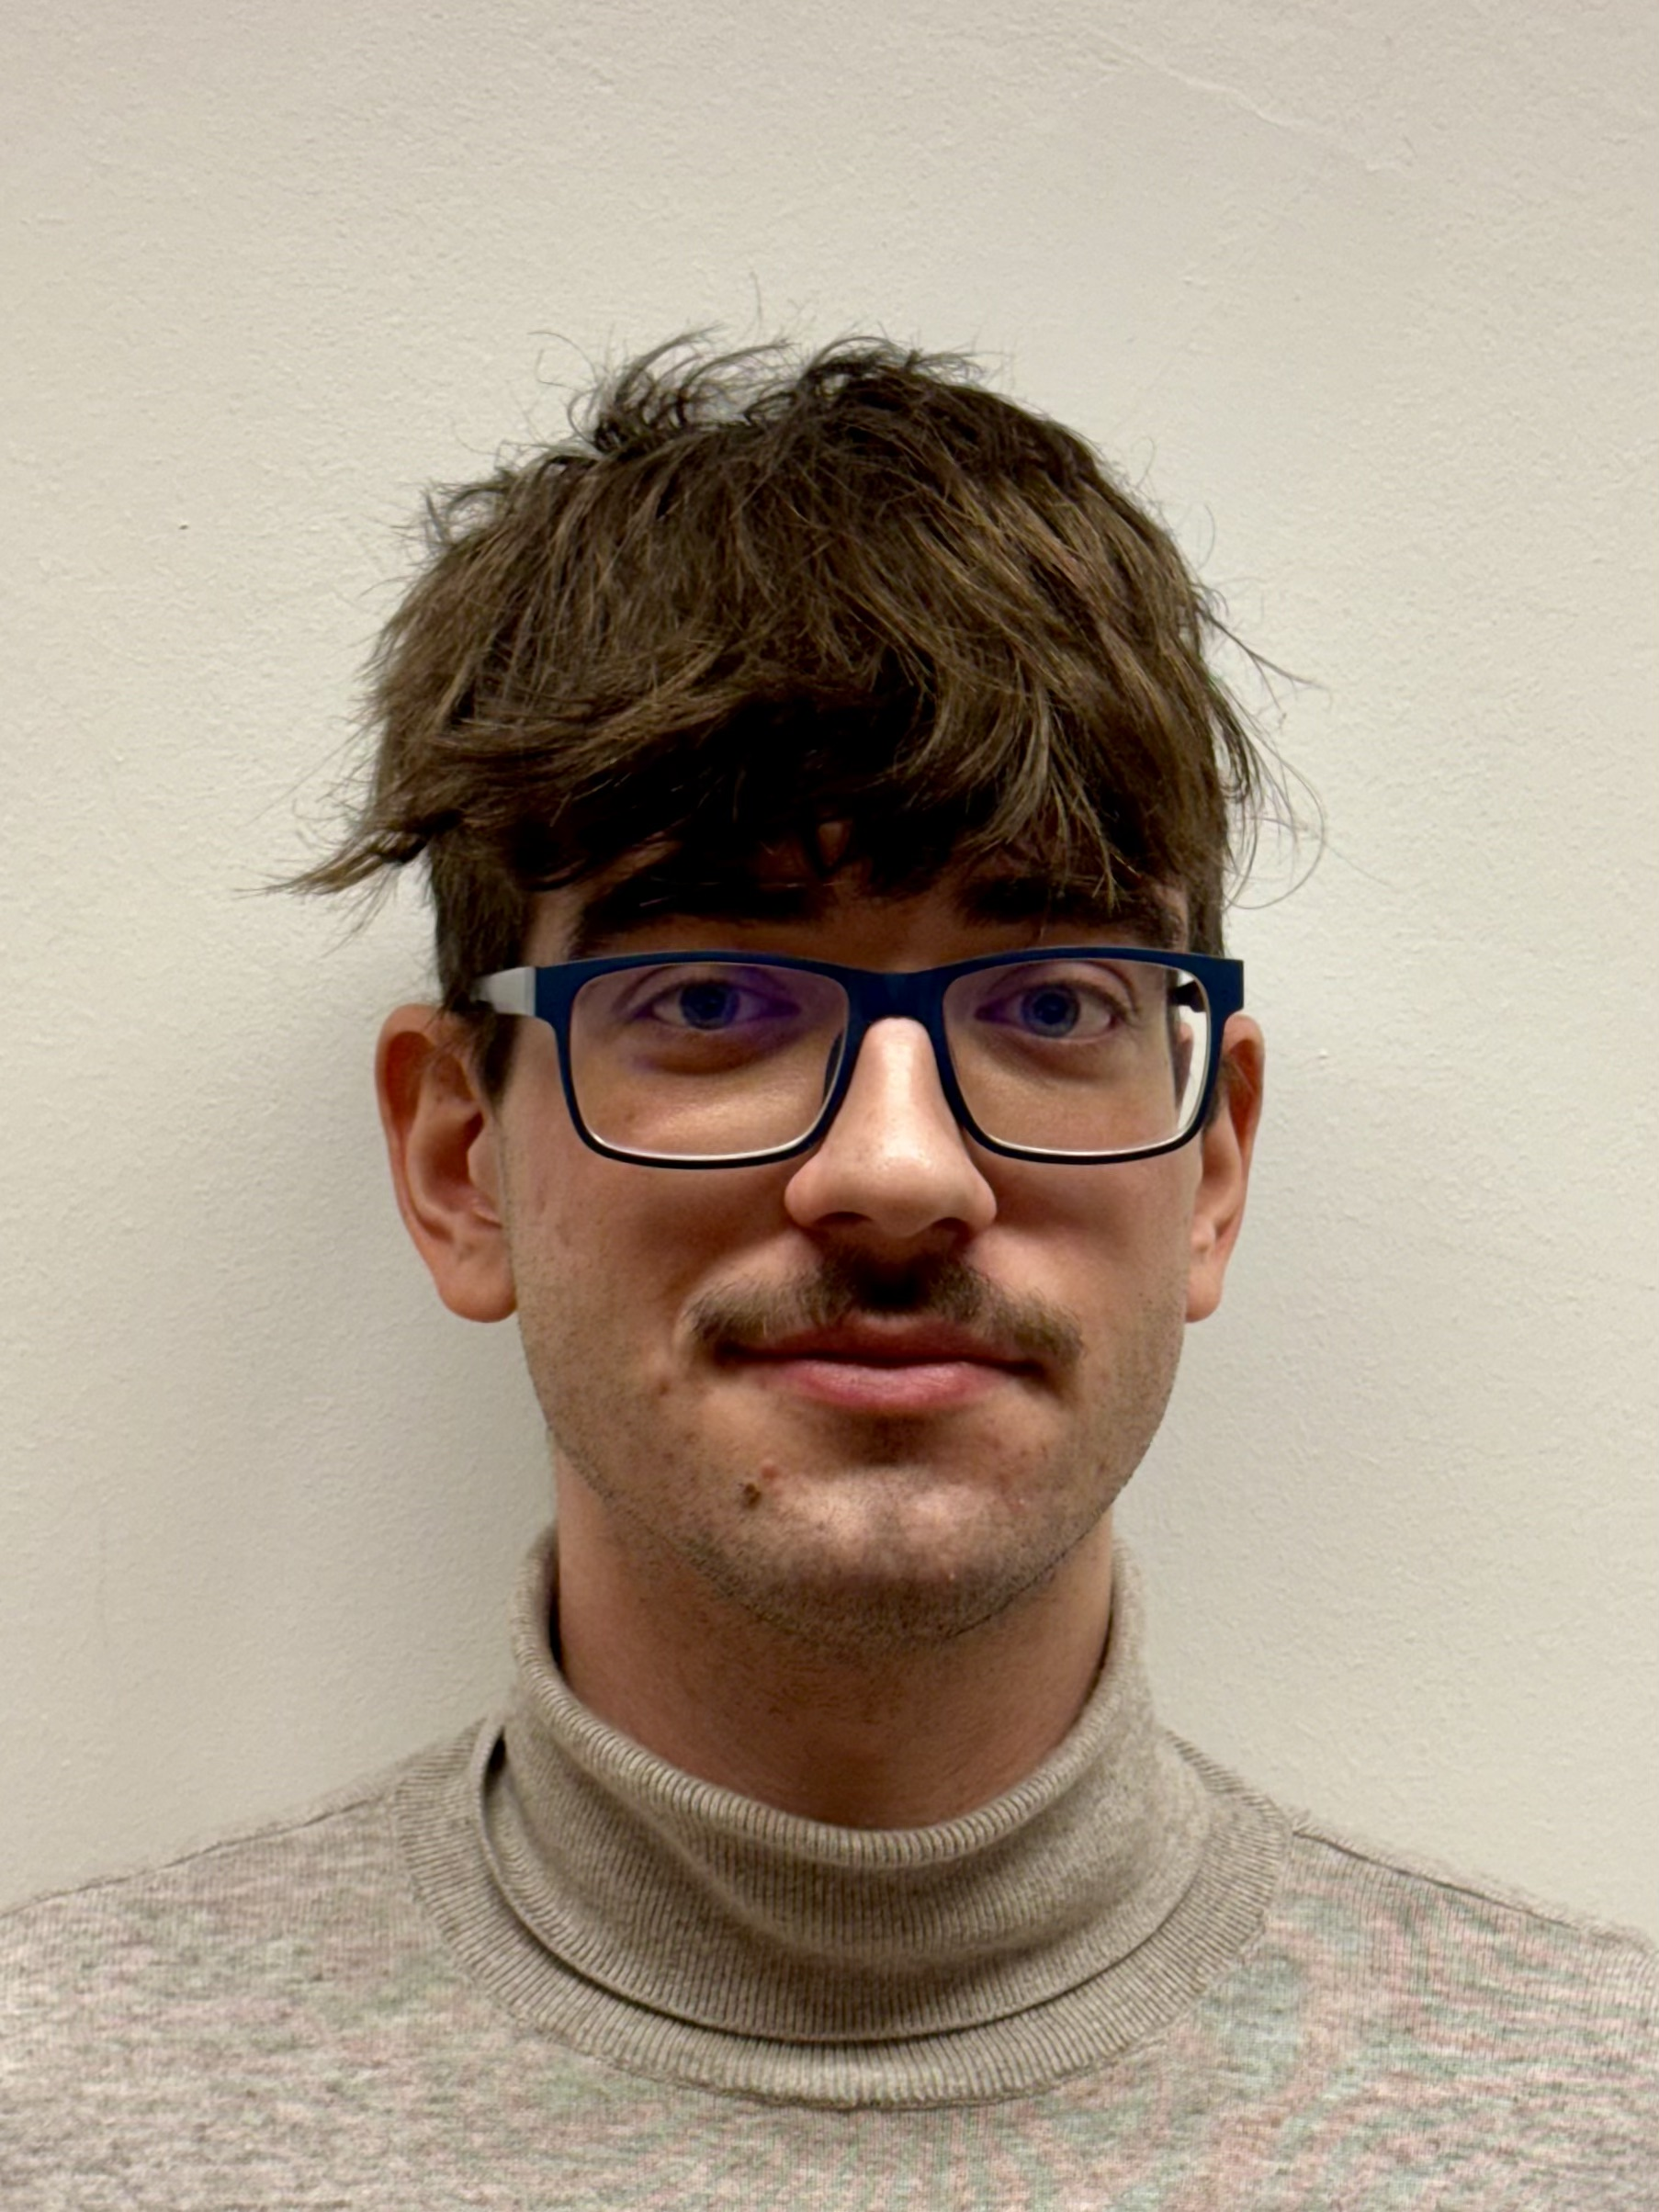
\includegraphics[width=\textwidth]{./static/visa-2024.jpeg}
	\vspace{.33em}

	%%% ---------------------------------------------------------------------- %%%
	\resumesection{Contact Information}

	\bgroup
	\addtolength{\tabcolsep}{-3pt}
	\def\arraystretch{1.25}
	\begin{tabular}{ll}
		\faCalendar  & Dec 20, 2001                 \\
		\faEnvelopeO & tiborsandor2001@gmail.com    \\
		\faPhone     & +36\,30\,298\,5235           \\
		\faBuildingO & 1119, Budapest, Etele út 18. \\
	\end{tabular}
	\egroup
	\vspace{1em}

	%%% ---------------------------------------------------------------------- %%%
	\resumesection{Soft Skills}

	\bgroup
	\addtolength{\tabcolsep}{-3pt}
	\def\arraystretch{1.25}
	\begin{tabular}{>{\bfseries}l}
		Communication       \\
		Problem-solving     \\
		Teamwork            \\
		Attention to detail \\
	\end{tabular}
	\egroup
	\vspace{1em}

	%%% ---------------------------------------------------------------------- %%%
	\resumesection{Language Knowledge}

	\bgroup
	\addtolength{\tabcolsep}{-3pt}
	\def\arraystretch{1.25}
	\begin{tabular}{>{\bfseries}l l}
		Hungarian & Native language  \\
		English   & B2 Language Exam \\
		German    & C1 Language Exam \\
	\end{tabular}
	\egroup
	\vspace{1em}

	%%% ---------------------------------------------------------------------- %%%
	\resumesection{Hobbies}

	\bgroup
	\addtolength{\tabcolsep}{-3pt}
	\def\arraystretch{1.25}
	\begin{tabular}{>{\bfseries}l}
		Traveling             \\
		Languages             \\
		Retro gaming consoles \\
	\end{tabular}
	\egroup
	\vspace{1em}

	%%% ---------------------------------------------------------------------- %%%
	\resumesection{Other}

	\bgroup
	\addtolength{\tabcolsep}{-3pt}
	\def\arraystretch{1.25}
	\begin{tabular}{>{\bfseries}l}
		Category B driving license
	\end{tabular}
	\egroup
	\vspace{1em}

	%%% ---------------------------------------------------------------------- %%%
	\resumesection{LinkedIn}

	\vfill

	\centering
	\qrcode[height=.5\textwidth, hyperlink]{https://www.linkedin.com/in/tibi1220}

	\vfill

	~
\end{minipage}\hfill%
%%% ------------------------------------------------------------------------ %%%
%%% ----------------------------- Right Column ----------------------------- %%%
%%% ------------------------------------------------------------------------ %%%
\begin{minipage}[b]{\rightcolumnwidth}
	% Motivation
	\resumesection{Motivation}

	As a mechatronics graduate student, I am excited to apply my acquired
	knowledge in a work environment, contributing to innovative solutions and
	gaining practical experience.

	\vspace{1em}

	%%% ---------------------------------------------------------------------- %%%
	\resumesection{Work Experience}

	\timedentry{Front-End Developer Intern, Actegon Solutions Kft}{2024}{2024}
	\begin{itemize}
		\item Project:
		      Rewriting a clinic's internal management software

		\item Stack:
		      React Front-End, GraphQL Back-End, Postgres DB

		\item Responsibilities:
		      \vspace{-2.85pt}\begin{itemize}
			      \item Creating a new UI interface based on the client's requirements
			      \item Displaying data in interactive tables
			      \item Implementing forms with validation and error handling
		      \end{itemize}
	\end{itemize}

	\timedentry{Teaching Assistant, BME}{2022}{}
	\begin{itemize}
		\item Teaching Calculus for students
		      (practical classes, first three semesters)
		\item Administering and grading midterms and final exams
		\item Publications in the field of Mathematics Education
		      \vspace{-2.85pt}\begin{itemize}
			      \item Presented a paper${}^1$ at the SEFI2024 international conference
		      \end{itemize}
	\end{itemize}

	\vspace{1em}

	%%% ---------------------------------------------------------------------- %%%
	\resumesection{Studies}

	\timedentry{Mechatronics MSc, BME}{2024}{}
	\begin{itemize}
		\item Specialization: Embedded Systems
		\item Expected graduation: 2026, currently in 2nd semester
		\item Would prefer to write my thesis at a company
		\item Current subjects include: Machine Vision
		      \vspace{-3pt}\begin{itemize}
			      \item Project: Designing a license plate recognition system
		      \end{itemize}
	\end{itemize}

	\timedentry{Mechatronics BSc, BME}{2020}{2024}
	\begin{itemize}
		\item Specialization: Design of Smart Devices
		\item Graduated with highest honors, GPA: 4.96
		\item Member of the "Department of Mechatronics" self organized group
	\end{itemize}

	\timedentry{Révai Miklós High School}{2016}{2020}
	\begin{itemize}
		\item Specialization: Mathematics and Physics,
		      GPA: 5.0

		\item Higher level final exam in Physics and English,
		      Average: 96\%
	\end{itemize}

	\vspace{1em}

	%%% ---------------------------------------------------------------------- %%%
	\resumesection{Computer Skills}

	\def\tspace{2.25cm}

	\textbf{Programming Languages}:

	\begin{itemize}
		\item \textbf{General}:
		      \tabto{\tspace}
		      \texttt{C},
		      \texttt{C++},
		      \texttt{Python},
		      \texttt{\LaTeX}

		\item \textbf{Linux}:
		      \tabto{\tspace}
		      \texttt{git},
		      \texttt{zsh},
		      \texttt{vim},
		      \texttt{docker}

		\item \textbf{Web}:
		      \tabto{\tspace}
		      \texttt{javascript},
		      \texttt{typescript},
		      \texttt{react},
		      \texttt{html},
		      \texttt{css},
		      \texttt{tailwindcss}

		\item \textbf{Cloud}:
		      \tabto{\tspace}
		      \texttt{Amazon Web Services}
	\end{itemize}

	\textbf{Programs}:

	\begin{itemize}
		\item \textbf{General}:
		      \tabto{\tspace}
		      Microsoft Office,
		      Adobe Photoshop,
		      Adobe Illustrator

		\item \textbf{Engineering}:
		      \tabto{\tspace}
		      SOLIDWORKS,
		      KiCad,
		      MPLAB,
		      LabVIEW,
		      MATLAB
	\end{itemize}
	\vspace{-6.65pt}
\end{minipage}
\end{document}
